\documentclass[a4paper]{article}
\usepackage[spanish]{babel}
\usepackage[utf8]{inputenc}
\usepackage{charter}   % tipografia
\usepackage{graphicx}
\usepackage{wrapfig}
%\usepackage{makeidx}

%\usepackage{float}
%\usepackage{amsmath, amsthm, amssymb}
%\usepackage{amsfonts}
%\usepackage{sectsty}
%\usepackage{charter}
%\usepackage{wrapfig}
%\usepackage{listings}
%\lstset{language=C}


\usepackage{color} % para snipets de codigo coloreados
\usepackage{fancybox}  % para el sbox de los snipets de codigo

\definecolor{litegrey}{gray}{0.94}

% \newenvironment{sidebar}{%
% 	\begin{Sbox}\begin{minipage}{.85\textwidth}}%
% 	{\end{minipage}\end{Sbox}%
% 		\begin{center}\setlength{\fboxsep}{6pt}%
% 		\shadowbox{\TheSbox}\end{center}}
% \newenvironment{warning}{%
% 	\begin{Sbox}\begin{minipage}{.85\textwidth}\sffamily\lite\small\RaggedRight}%
% 	{\end{minipage}\end{Sbox}%
% 		\begin{center}\setlength{\fboxsep}{6pt}%
% 		\colorbox{litegrey}{\TheSbox}\end{center}}

\newenvironment{codesnippet}{%
	\begin{Sbox}\begin{minipage}{\textwidth}\sffamily\small}%
	{\end{minipage}\end{Sbox}%
		\begin{center}%
		\colorbox{litegrey}{\TheSbox}\end{center}}



\usepackage{fancyhdr}
\pagestyle{fancy}

%\renewcommand{\chaptermark}[1]{\markboth{#1}{}}
\renewcommand{\sectionmark}[1]{\markright{\thesection\ - #1}}

\fancyhf{}

\fancyhead[LO]{Sección \rightmark} % \thesection\ 
\fancyfoot[LO]{\small{Ituarte Joaquin, Maddonni Axel, Oller Luca}}
\fancyfoot[RO]{\thepage}
\renewcommand{\headrulewidth}{0.5pt}
\renewcommand{\footrulewidth}{0.5pt}
\setlength{\hoffset}{-0.8in}
\setlength{\textwidth}{16cm}
%\setlength{\hoffset}{-1.1cm}
%\setlength{\textwidth}{16cm}
\setlength{\headsep}{0.5cm}
\setlength{\textheight}{25cm}
\setlength{\voffset}{-0.7in}
\setlength{\headwidth}{\textwidth}
\setlength{\headheight}{13.1pt}

\renewcommand{\baselinestretch}{1.1}  % line spacing


% \setcounter{secnumdepth}{2}
\usepackage{underscore}
\usepackage{caratula}
\usepackage{url}
\usepackage{float}


% ******************************************************** %
%              TEMPLATE DE INFORME ORGA2 v0.1              %
% ******************************************************** %
% ******************************************************** %
%                                                          %
% ALGUNOS PAQUETES REQUERIDOS (EN UBUNTU):                 %
% ========================================
%                                                          %
% texlive-latex-base                                       %
% texlive-latex-recommended                                %
% texlive-fonts-recommended                                %
% texlive-latex-extra?                                     %
% texlive-lang-spanish (en ubuntu 13.10)                   %
% ******************************************************** %

\begin{document}


\thispagestyle{empty}
\materia{Organización del Computador II}
\submateria{Primer Cuatrimestre de 2015}
\titulo{Trabajo Práctico II}
\subtitulo{Modelo SIMD}
\grupo{Grupo Crash Bash/Ps1}
\integrante{Ituarte, Joaquin}{457/13}{joaquinituarte@gmail.com} % obligatorio 
\integrante{Maddonni, Axel}{200 /14}{axel.maddonni@gmail.com} % obligatorio 
\integrante{Oller, Luca}{667/13}{ollerrr@live.com} % obligatorio 

\maketitle
\newpage

\thispagestyle{empty}
\vfill

\thispagestyle{empty}
\vspace{3cm}
\tableofcontents
\newpage

%\normalsize
\newpage

\section{Introducción}

En este trabajo se presentan y comparan tres implementaciones, dos en Assembler y una en C,  para la realización de tres filtros de imágenes. Estos filtros son el filtro Blur, el filtro Merge y el filtro HSL.

Las imágenes que utilizamos son múltiplos de cuatro y mayores a 16x16.

El filtro Blur toma una imagen y la suaviza, el filtro Merge toma dos imágenes del mismo tamaño y las mezcla en una sola imagen, mientras que el filtro HSL convierte los píxeles RGB a HSL, una vez convertidos se los modifica y finalmente los píxeles regresan a RGB. 

La primera parte del trabajo tratará de exponer y explicar el funcionamiento de cada una de las implementaciones en assembler de forma individual. Luego, desarrollaremos una comparación entre ellas analizando las ventajas y desventajas, exponiendo en qué casos es conveniente utilizar una u otra dependiendo del contexto de uso, cuáles son las causas y qué maneras hay de optimizarlas.

Al finalizar las explicaciones, se detallarán además las conclusiones obtenidas y las problemáticas que se nos presentaron  en la realización del trabajo práctico.

\newpage

\section{Desarrollo} 

\subsection{Blur}

\subsubsection{Implementacion 1}

\textbf{Explicación assembler}

En esta implementación modificamos de a un pixel a la vez, comenzando a recorrer la primer fila de la matriz que representa a la imagen hasta que ésta se acabe y luego repetir el proceso con la fila siguiente hasta alcanzar el borde cuyos píxeles no son modificados. Para calcular los valores resultantes de cada componente del pixel, mantenemos en cada iteración un puntero al primero de los 9 píxeles necesarios para el cálculo correspondiente al filtro Blur (ver enunciado).

Para poder calcular correctamente los píxeles, debemos tener cuidado de no utilizar el valor modificado de los píxeles vecinos que utilizamos para realizar las cuentas.

Para lograr lo dicho anteriormente, al comienzo del código creamos un vector del tamaño equivalente a una fila de la imagen, que lo vamos a utilizar para guardar temporalmente n píxeles, siendo n la cantidad de píxeles que tiene una fila.

Este vector lo inicializamos con los píxeles de la primera fila de la imagen. Aunque ésto no es necesario, de esta manera nos evitamos realizar el caso base correspondiente a la primera fila de la imagen, ya que ésta no se modifica, fuera del ciclo correspondiente.

Nuestra función opera de la siguiente manera:
Hay dos ciclos, uno dentro del otro, en donde el ciclo externo itera sobre las filas y el ciclo interno lo hace sobre las columnas.

\begin{figure}[ht!]
\centering
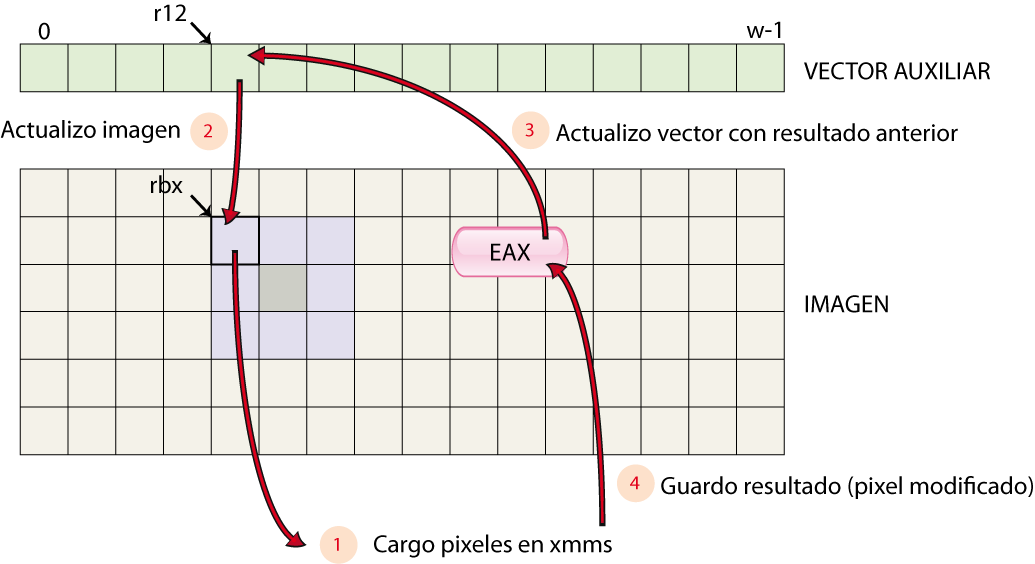
\includegraphics[width=120mm]{imagenes/blur/blur1-figura1.png}
\caption{Desarrollo de Blur-ASM1.}
\end{figure}

1) En el ciclo interno guardamos en 3 registros xmm, en nuestro caso xmm0, xmm2 y xmm4, los primeros cuatro píxeles consecutivos de 3 filas contiguas. De estos 4 píxeles vamos a necesitar solamente 3, de forma que los píxeles que utilicemos sean los píxeles vecinos al pixel que vamos a modificar y a si mismo.

\begin{figure}[ht!]
\centering
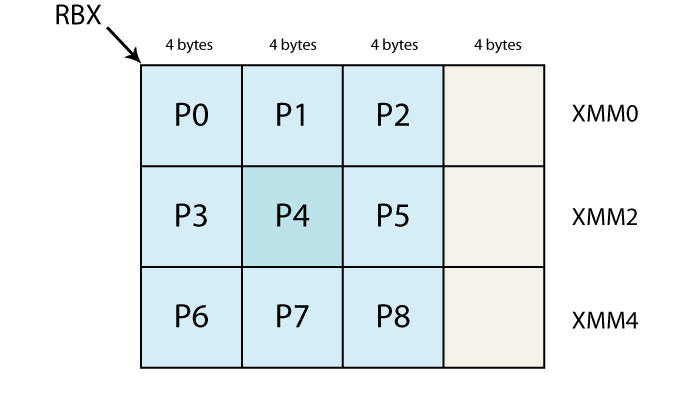
\includegraphics[width=70mm]{imagenes/blur/blur1-figura2.png}
\caption{Desarrollo de Blur-ASM1.}
\end{figure}

2) Una vez que los píxeles de la imagen están en los registros, modificamos el pixel de la imagen ubicado en la menor posición intercambiándolo con el pixel correspondiente del vector creado previamente, que contiene el pixel ya modificado correspondiente a esa posición de memoria.

3) Ahora que ya utilizamos la posición del vector para actualizar la imagen, guardamos el resultado que habíamos obtenido en la iteración anterior (que guardamos en EAX) en el vector. En caso que sea el primer pixel de la fila, antes de entrar al ciclo de la nueva fila se guarda en EAX el pixel correspondiente.

4) Realizamos las operaciones necesarias con los datos y guardamos el resultado (el pixel modificado) en EAX.
Para sumar las componentes de los píxeles sin que ocurra overflow en nuestra representación, duplicamos el tamaño de cada una de ellas expandiendolas de byte a word. Dejamos dos píxeles en el registro en el que estaban (con el tamaño modificado) y los otros dos en otro registro xmm. 
Luego realizamos suma de words entre los registros, el resultado lo guardamos en xmm0. 
El siguiente paso es  shiftear a la derecha los registros xmm0, xmm2 y xmm4 y los sumamos para asi obtener en la parte baja del registro xmm0 la suma de los 9 pixeles involucrados.
Duplicamos el tamaño de cada componente a 32 bits para convertir a float y dividir por nueve cada uno de ellos. Una vez concluído ésto, volvemos a convertir las componentes a enteros, y volvemos a empaquetarlas a su tamaño original, de forma que quede el pixel resultante en la parte más baja del registro xmm0.
El resultado obtenido lo guardo en un registro para poder ubicarlo en el vector en la iteración siguiente. No lo podemos guardar en el vector ahora porque todavía necesitamos usar el valor correspondiente a esa posición en la próxima iteración.

\begin{figure}[ht!]
\centering
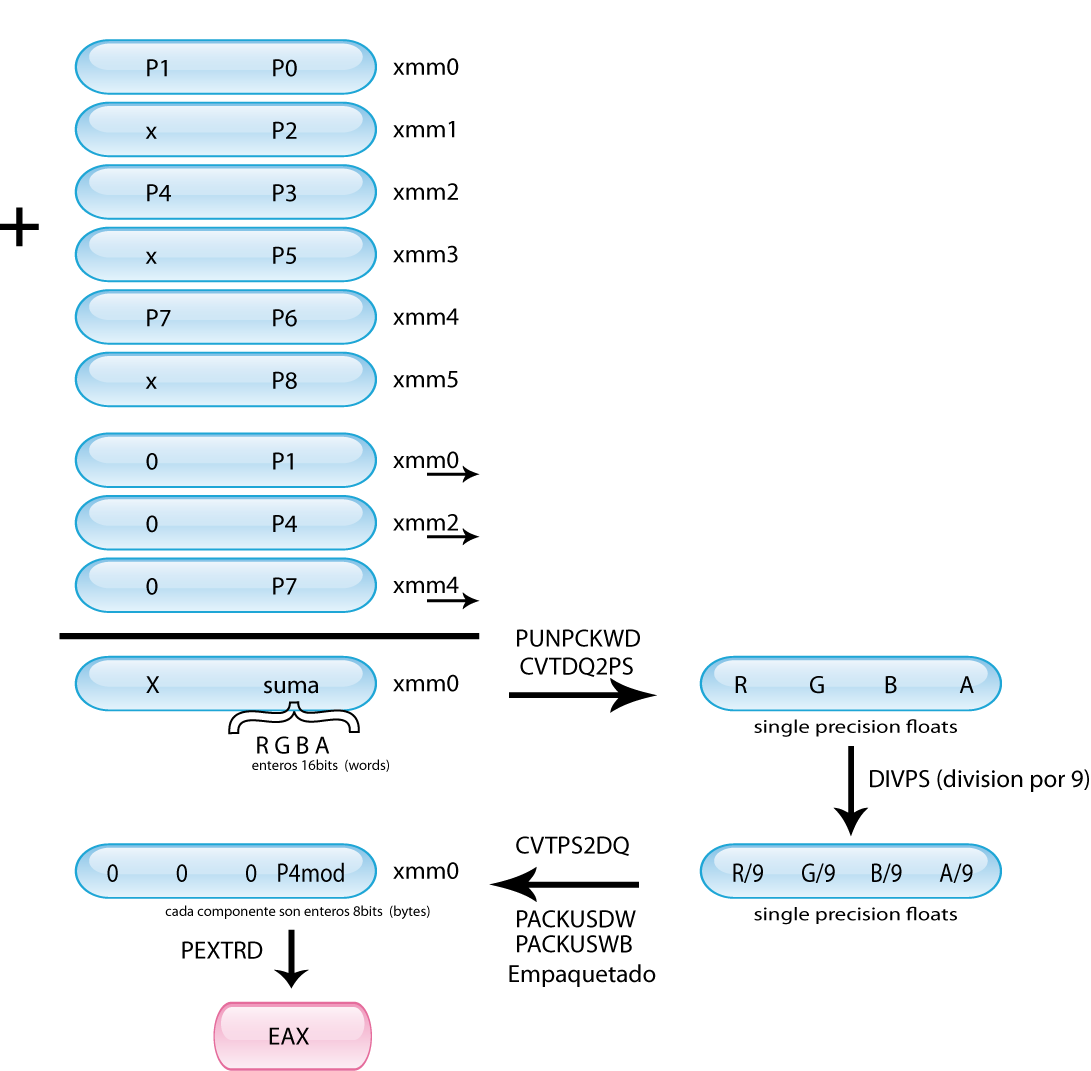
\includegraphics[width=100mm]{imagenes/blur/blur1-figura3.png}
\caption{Desarrollo de Blur-ASM1.}
\end{figure}

Caso Borde: Antes de volver a iterar en el ciclo externo, se realiza el caso borde del final de la fila, que es análogo a una iteración del ciclo interno. Cuando se llega a la última columna de pixeles que se debe modificar, retrocedemos con el puntero al pixel anterior y tomamos los ultimos 3 pixeles de cada registro en vez de los 3 primeros. (Si no hariamos ésto, en la ultima fila intentariamos acceder a memoria que no es nuestra).
Nota: Al finalizar el caso borde actualizamos el anteúltimo pixel de la fila y cargamos el resultado directo al vector, no hace falta guardarlo en EAX.

Una vez finalizado ésto, realizamos las operaciones necesarias para poder realizar la siguiente iteración del ciclo externo.

Al finalizar el ciclo de las filas, actualizamos la anteúltima fila con los valores modificados, guardados en el vector durante la última iteración del ciclo.


\subsubsection{Implementacion 2}

\textbf{Explicación assembler}

En esta implementación modificamos la imagen de a cuatro píxeles por vez, considerando a la imagen como una matriz de píxeles. El orden que seguimos para procesar los grupos de píxeles es: procesar los primeros cuatro píxeles de la imagen (sin contar los bordes) y hacer lo mismo con el siguiente grupo de píxeles hasta que llegamos al final de la fila, donde debemos procesar solo dos píxeles. Luego cambiamos de fila y repetimos el proceso hasta llegar a la última fila de la imagen.

Para lograr ésto debemos tener cuidado de no procesar píxeles con los valores modificados de sus vecinos. Al igual que en la anterior implementación, utilizamos un vector del tamaño de una fila de la matriz en donde guardaremos los valores modificados de la imagen hasta que hayamos utilizado a los píxeles que se deben reemplazar en todas las cuentas en las que se vean implicados.
Este vector es inicializado con los píxeles correspondientes a la primera fila de la imagen para evitar problemas en la primer iteración del ciclo cuando actualizamos la imagen.

\begin{figure}[ht!]
\centering
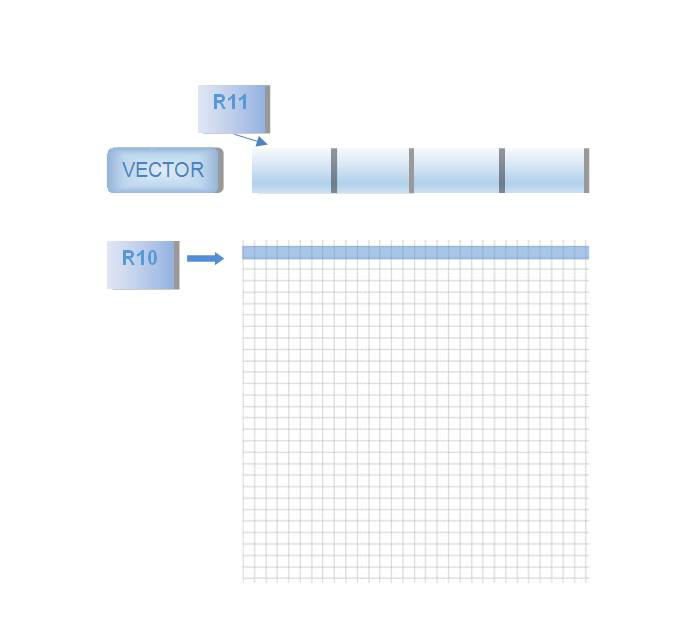
\includegraphics[width=90mm]{imagenes/blur/blur2-1.png}
\caption{Desarrollo de Blur-ASM2.}
\end{figure}

Luego de haber inicializado el vector, comenzamos con los ciclos para el procesamiento de los píxeles utilizando dos ciclos: un ciclo externo que recorre las filas y un ciclo interno que recorre las columnas, contenido por el primero.

Al comenzar el ciclo externo, inicializamos los registros para manipular los datos que se van a utilizar en el ciclo interno. Estos datos son el ancho de la fila, que es nuestra referencia a cantidad de iteraciones a realizar en el ciclo interno, un puntero a la dirección de memoria del primero de todos los píxeles que vamos a utilizar, y un puntero al inicio del vector.

Luego comienza a realizarse el ciclo interno.

Al comenzar el ciclo interno, utilizamos nueve registros xmm para guardar los grupos de cuatro píxeles de la siguiente forma:

\begin{figure}[ht!]
\centering
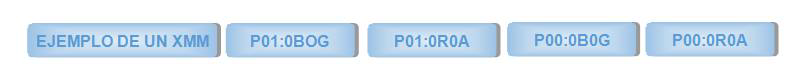
\includegraphics[width=120mm]{imagenes/blur/blur2-2.png}
\caption{Desarrollo de Blur-ASM2.}
\end{figure}

Una vez cargados los píxeles en los registros, procedemos a actualizar los cuatro píxeles de la imagen original con los cuatro píxeles correspondientes al vector creado. Es decir, actualizamos el valor de los píxeles que ya terminamos de utilizar, y de manera análoga a la implementación 1, cargamos en el vector el cuarto de los 4 pixeles que habíamos calculado en la iteración anterior y guardado en un registro, para no pisar los valores que necesitamos para actualizar la imagen.

Paso siguiente es duplicar el tamaño de las componentes de los píxeles en los registros xmm utilizados previamente. Como los registros ahora pasan a poder contener solamente dos píxeles, vamos a necesitar el doble de registros para poder guardar todos los píxeles necesarios.

\begin{figure}[ht!]
\centering
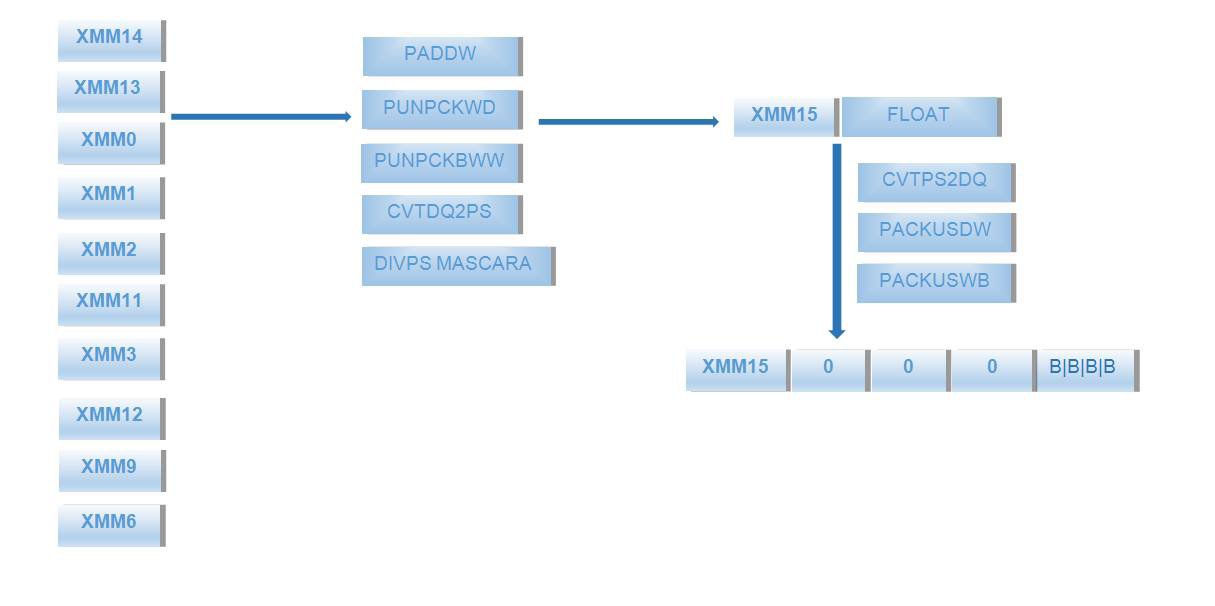
\includegraphics[width=120mm]{imagenes/blur/blur2-3.png}
\caption{Desarrollo de Blur-ASM2.}
\end{figure}

A continuación, realizamos las operaciones para calcular un pixel. Hacemos la sumatoria de las componentes de los píxeles, guardando el resultado en otro registro, transformamos ese resultado a punto flotante de precisión simple para poder divirlas a todas a la vez y obtener el promedio. Una vez calculado, lo transformamos nuevamente a entero.

Una vez calculado el pixel, lo transformo a su tamaño original, y copio el pixel al vector creado al comienzo del código. 

\begin{figure}[ht!]
\centering
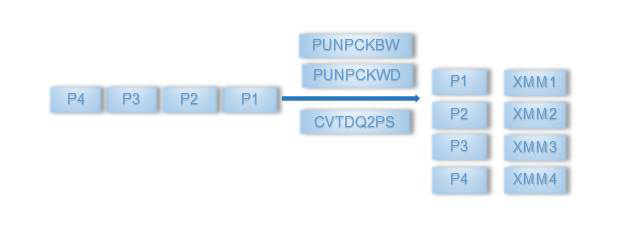
\includegraphics[width=100mm]{imagenes/blur/blur2-4.png}
\caption{Desarrollo de Blur-ASM2.}
\end{figure}

Para calcular los otros tres píxeles, el procedimiento es similar al recién descrito, teniendo en cuenta la ubicación de los píxeles necesarios en los registros utilizados. El cuarto pixel, como se menciona antes, se guarda provisoriamente en un registro pues el valor que le correspondería en el vector sera utilizado al comienzo del próximo ciclo.

Al finalizar el ciclo interno, debemos procesar los últimos dos píxeles de la fila iterada debido a que el ciclo sólo procesa de a cuatro píxeles. Este procesamiento es análogo a una iteración del ciclo interno, pero manipulando con precaución los registros debido a que usamos menor cantidad de píxeles y de cantidad de registros xmm.

Finalizado el procesamiento de estos dos píxeles, cambiamos la fila que vamos a iterar en el ciclo interno de la siguiente iteración del ciclo externo.

El ciclo externo termina cuando no hay más filas de la imagen que procesar, dejando las últimas dos filas de la imagen sin modificar, y las modificaciones de la anteúltima fila de la misma imagen en el vector creado por nosotros.

Cuando termina de realizarse el ciclo externo, debemos copiar los datos del vector a la anteúltima fila de la imagen, y con esto finaliza la función.

\newpage

\subsection{Merge}

\subsubsection{Implementacion 1}

\textbf{Explicación Assembler}

En la primera implementación del filtro Merge, realizamos dos ciclos anidados los cuales iteran sobre la fila y sobre las columnas de la matriz de la imagen respectivamente, similar a las implementaciones anteriores. En el ciclo que itera sobre las columnas, iteramos de a cuatro píxeles, recorriendo toda una fila dictada por el otro ciclo. Estos punteros se manipulan de manera análoga para ambas imágenes, dado que éstas tienen que ser de iguales dimensiones.

Al llegar al final de una fila, es decir, cuando el ciclo de las columnas termina, actualizamos los punteros de las imágenes sumándole al puntero el tamaño de la fila para cambiar a la siguiente, y realizamos las iteraciones hasta terminar de operar con todas las filas de la imagen.

\begin{figure}[ht!]
\centering
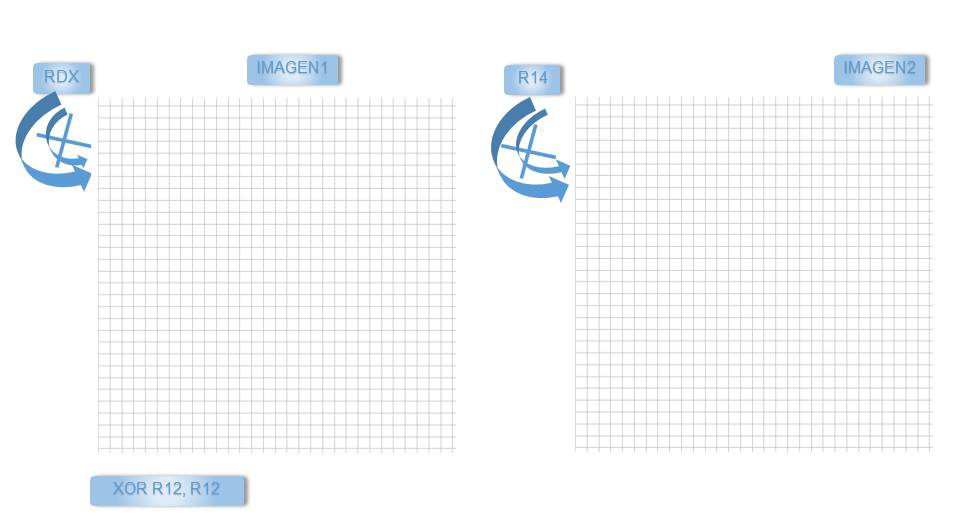
\includegraphics[width=100mm]{imagenes/merge/merge1-1.png}
\caption{Desarrollo de Merge-ASM1.}
\end{figure}

Dentro del ciclo de las columnas guardamos en dos registros xmm los cuatro píxeles de cada imagen. Luego desempaquetamos cada registro en otros dos registros para incrementar el tamaño de las componentes de los píxeles y volvemos a repetir esta operación para obtener cada pixel ocupando un registro xmm, una componente por doubleword, y así convertirlos a float.

%\begin{figure}[ht!]
%\centering
%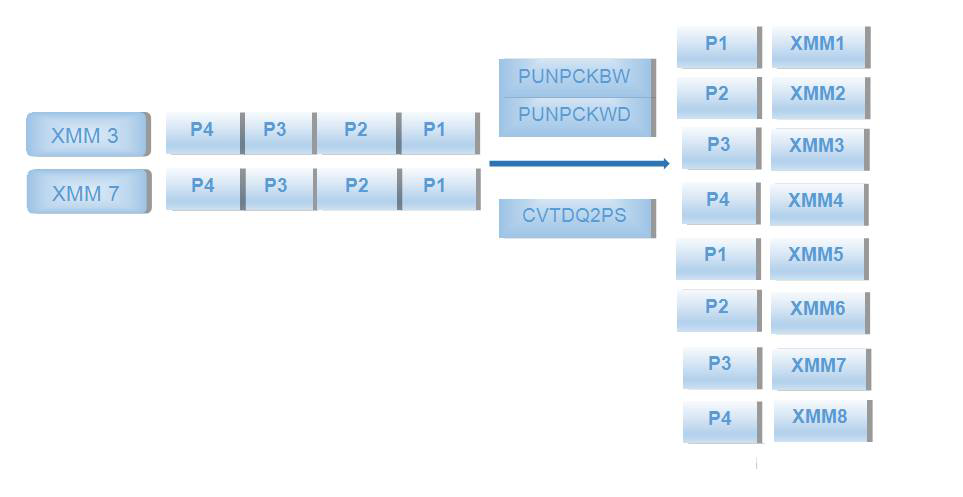
\includegraphics[width=90mm]{imagenes/merge/merge1-2.png}
%\caption{*************INSERTAR IMAGEN DE LOS XMM CORRESPONDIENTES CON LAS LOS PIXELES*************}
%\end{figure}

Luego realizamos el producto del RGB del píxel por nuestro value, dejando intacto A, y al píxel ubicado en la misma posición pero en la otra imagen hacemos el producto por 1-value. A estos valores los sumamos y convertimos a enteros, y los empaquetamos de dword a word y de word a byte para que el píxel recupere su valor original.

\begin{figure}[ht!]
\centering
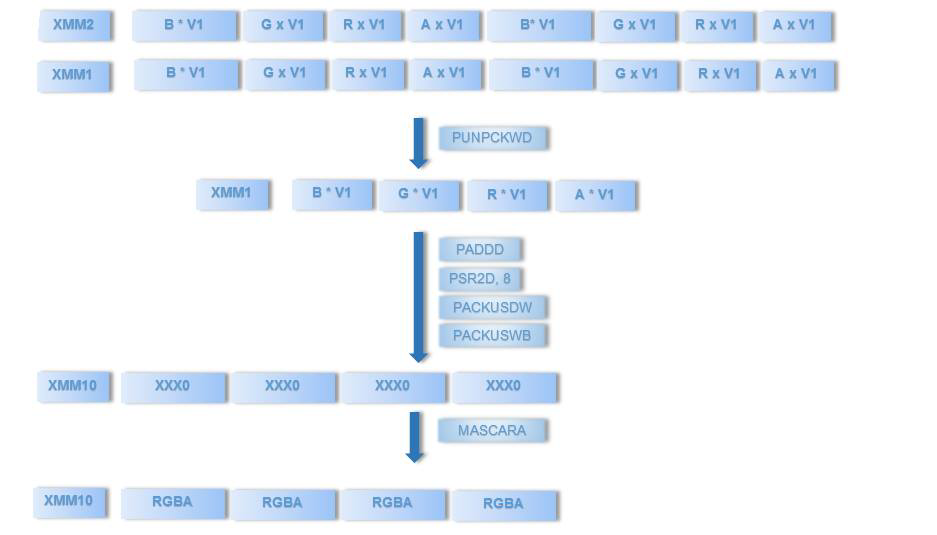
\includegraphics[width=120mm]{imagenes/merge/merge1-3.png}
\caption{Desarrollo de Merge-ASM1.}
\end{figure}

Para finalizar, volvemos a guardar el pixel en memoria y termino de realizar la iteración, para volver a comenzar a repetir el proceso con los siguientes 4 píxeles.

\subsubsection{Implementacion 2}

\textbf{Explicacion Assembler}

En la segunda implementación del filtro Merge realizamos la implementación utilizando números enteros. Como value es un float entre 0 y 1, debimos encontrar una forma de manipular la función para que use valores en entero. Por ésto, debemos multiplicar a value por 256 y guardamos su valor y su complemento en los registros XMM0 y XMM15 con tamaño word en todas las posiciones posibles de los registros. Elegimos el valor 256, ya que luego al momento de dividir, al ser una potencia de 2 nos facilita la tarea. Además, tuvimos en cuenta de no pasarnos del valor máximo posible dado la cantidad de bits de un word, al momento de realizar las operaciones, para que no se produzca overflow.

\begin{figure}[ht!]
\centering
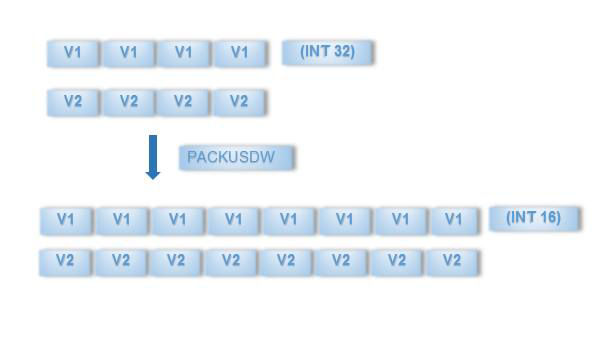
\includegraphics[width=90mm]{imagenes/merge/merge2-1.png}
\caption{Desarrollo de Merge-ASM2.}
\end{figure}

Después de realizar esta manipulación de los datos, comenzamos a operar usando 2 ciclos anidados, copiando cuatro píxeles de cada imagen los registros xmm1 y xmm5 en cada iteración. En un tercer registro, en nuestro caso xmm10, guardamos la componente A de cada pixel ya que no debe ser modificada. Luego duplicamos el tamaño de las componentes de los píxeles de xmm1 y xmm5 y guardamos 2 píxeles por registro, usando además los registros xmm3 y xmm7 para poder contenerlos a todos.

A continuación procedemos a multiplicar los píxeles de los registros por value o su complemento, dependiendo a que imagen pertenecen, expandiendo el tamaño de las componentes de los resultados obteniendo los siguientes registros:

\begin{figure}[ht!]
\centering
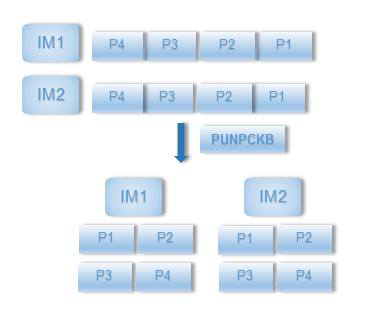
\includegraphics[width=70mm]{imagenes/merge/merge2-2.png}
\caption{Desarrollo de Merge-ASM2.}
\end{figure}

Una vez obtenidos los píxeles de esta forma, procedemos a realizar la suma de los píxeles de una imagen con los correspondientes de la otra, y dividimos cada componente por 256 (el valor utilizado al inicio para poder operar con enteros). Esta división la realizamos utilizando PSRLD XMMi, 8, que es equivalente a dividir cada componente por 256.

Finalizadas estas operaciones, continuamos por volver las componentes de los píxeles a su tamaño original, guardando los 4 píxeles en XMM1, y restaurando el valor de la componente A que habiamos guardado en XMM10.

\begin{figure}[ht!]
\centering
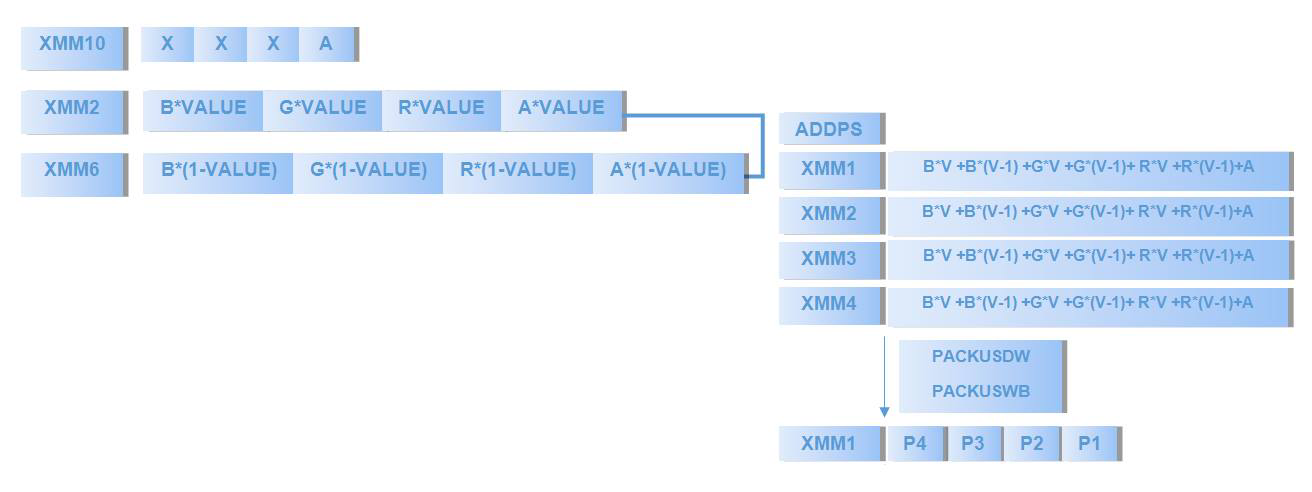
\includegraphics[width=140mm]{imagenes/merge/merge2-3.png}
\caption{Desarrollo de Merge-ASM2.}
\end{figure}

Luego de terminar con las operaciones, guardo en memoria los píxeles modificados y repito las operaciones con los siguientes 4 hasta procesarlos a todos.

\newpage

\subsection{HSL}

\subsubsection{Implementacion 1}

\textbf{Explicación Assembler}

La matriz se recorre de manera análoga a las implementaciones anteriores, utilizamos dos ciclos, uno para recorrer las filas y otro las columnas.

Esta implementación utiliza llamados a funciones de C para la transformación de formatos del pixel.

Para realizar ésto, guardamos en cada doubleWord del registro XMM0 los valores pasados como parámetro en la función, que corresponden al dato a sumar a cada componente del pixel.
Además, creamos un vector en donde vamos a guardar el resultado de llamar a la función para transformar un pixel a formato HSL (utilizando una función C ya implementada).

\begin{figure}[ht!]
\centering
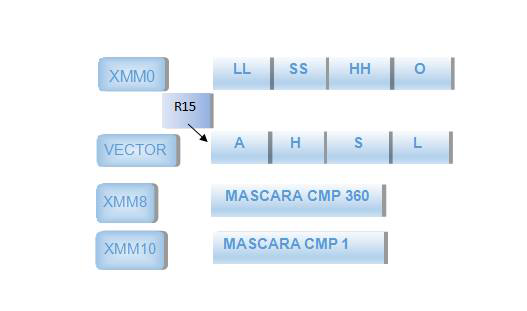
\includegraphics[width=80mm]{imagenes/hsl/hsl1-1.png}
\caption{Desarrollo de HSL-ASM1.}
\end{figure}

Una vez realizado esto, procedemos a realizar las operaciones debidas a los píxeles iterando uno a uno todos los píxeles de la imagen.

En cada iteración comenzamos transformando las componentes del pixel rgb a componentes HSL con la función implementada en C correspondiente, usando el vector creado por nosotros como contenedor del resultado.

\begin{wrapfigure}{r}{70mm}
\centering
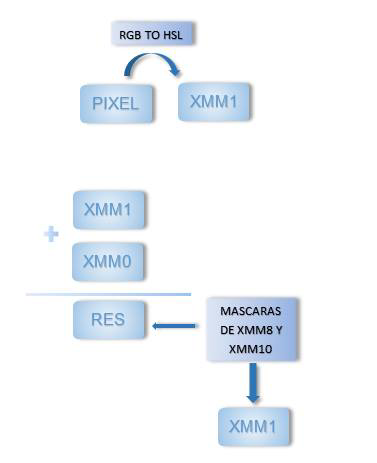
\includegraphics[width=70mm]{imagenes/hsl/hsl1-2.png}
\caption{Desarrollo de HSL-ASM1.}
\end{wrapfigure}

Una vez obtenido este resultado, lo cargamos en el registro XMM1 y le sumamos los datos correspondientes, que previamente habiamos guardado en XMM0. Luego controlamos que los valores obtenidos sean válidos y correctos según las fuciones dadas por la cátedra, implementando las funciones condicionales analizando si se cumplen las condiciones desde el final hacia el principio. Es decir, vemos si el último caso de la función condicional es válido. Si es válido, escribimos ese valor y procedemos a analizar el caso anterior de la función. Si también correcto cambiamos el valor escrito anteriormente por este, quedando como resultado final de la función el primer caso valido de la función.

Una vez finalizadas estas operaciones, guardamos el resultado en nuestro vector y procedemos a volver a convertir las componentes HSL a componentes rgb utilizando la función C correspondiente, la cual guarda el resultado final del pixel en la imagen.

Una vez terminadas todas las iteraciones, liberamos la memoria correspondiente a nuestro vector y terminamos la función.

\newpage

\subsubsection{Implementacion 2}

\textbf{Explicación Assembler}

En esta implementación realizamos el filtro HSL completamente en código assembler.

Para eso, realizamos la misma implementación de suma que la primera implementación del filtro explicada anteriormente.

Para realizar la conversión del formato rgb al formato HSL, transformamos el tamaño cada componente del pixel de byte a doubleword y las guardamos en el registro XMM0, los convertimos a valores en punto flotante y guardamos la componente de transparencia, dado que no se modifica, en el vector.

Calculamos el máximo y el mínimo entre las componentes rgb del pixel y con estos valores procedemos a calcular la matiz (componente H), luego la luminosidad (componente L) y finalmente la saturación (componente S) según las funciones dadas por la cátedra. Como las funciones para calcular las componentes son condicionales, hemos decidido realizar las operaciones desde el último caso hasta el primero, preguntando si las condiciones se cumplen, y reemplazando el valor anterior en caso de cumplirse. Esto ahorra ademas, comparar cada valor con el valor maximo y el minimo posible correspondiente a cada if. Luego, los resultados de estas operaciones son guardados en el vector.

\begin{figure}[ht!]
\centering
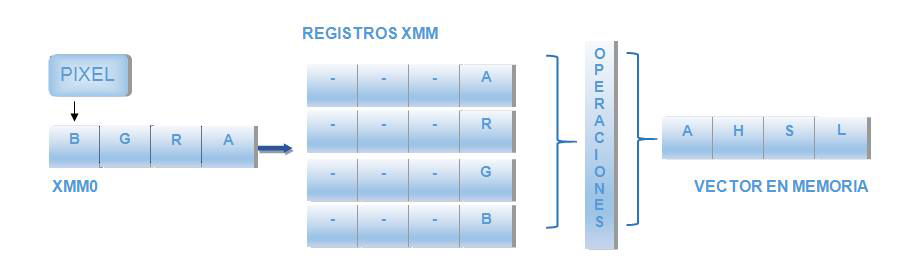
\includegraphics[width=130mm]{imagenes/hsl/hsl2-1.png}
\caption{Desarrollo de HSL-ASM2.}
\end{figure}

Para realizar la conversión del formato HSL al formato rgb, necesitamos obtener algunos valores utilizando las fórmulas provistas por la cátedra, C, X y M, que los guardaremos en las partes bajas de XMM4, XMM5 y XMM6 respectivamente. Para calcular fabs utilizamos una mascara que pone en 0 el bit de signo, mientras que para calcular fmod utilizamos divisiones y conversiones a enteros y nuevamente a float para eliminar los decimales y poder hacer el calculo como muestra la figura. Luego procedemos a calcular los valores en formato rgb según los resultados de las funciones condicionales otorgadas también por la cátedra, utilizando la misma lógica sobre las condiciones como se hizo anteriormente en la función para transformar de rgb a HSL. En cada if, utilizamos instrucciones de SHUFFLE para ir modificando en caso de que sea necesario, los valores de R, G y B. El resultado de ésto es guardado en XMM4 y luego hacemos los cálculos de escala (multiplicar todas las componentes por 255) y los convertimos a enteros.

\begin{figure}[ht!]
\centering
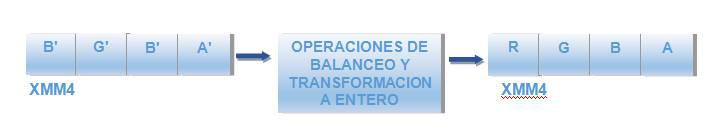
\includegraphics[width=100mm]{imagenes/hsl/hsl2-2.png}
\caption{Desarrollo de HSL-ASM2.}
\end{figure}

Para finalizar, volvemos las componentes a su tamaño original en la parte baja de XMM4 y lo guardamos en su posición original en la imagen.

\begin{figure}[ht!]
\centering
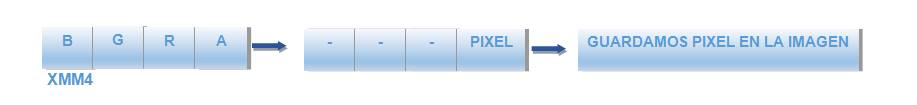
\includegraphics[width=130mm]{imagenes/hsl/hsl2-3.png}
\caption{Desarrollo de HSL-ASM2.}
\end{figure}


\newpage

\section{Resultados}

\subsection{Consideraciones sobre los tests}

\begin{itemize}

\item {Los tests que implementamos para medir el rendimiento de los programas fueron implementados en C utlizando las instrucciones de assembler RDTSC para obtener el valor del Time Stamp Counter y CPUID para evitar que el código que queremos medir se realice con ejecución fuera de orden. Esta instrucción sincrónica, la usamos entonces, para serializar la ejecución del código.}

\item {El código consiste en 1000 ejecuciones seguidas de las distintas implementaciones de los filtros, obteniendo los resultados con la cantidad de ciclos que tardo cada una de ellas en una planilla de excel .svc .}

\item {Para evitar, en parte, el overhead, decidimos modificar las funciones run_[nombre_del_filtro] provistas por la cátedra, de modo que se comience a medir los ciclos justo antes de llamar a la funcion que aplica el filtro, sin contar las operaciones sobre los bmp que realiza antes y despues del llamado a esta. }

\begin{figure}[ht!]
\centering
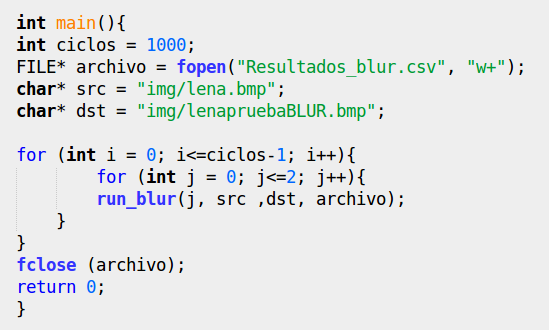
\includegraphics[width=90mm]{imagenes/resultados/codigoblur.png}
\caption{Código para testear rendimiento de Blur.}
\end{figure}

\begin{figure}[ht!]
\centering
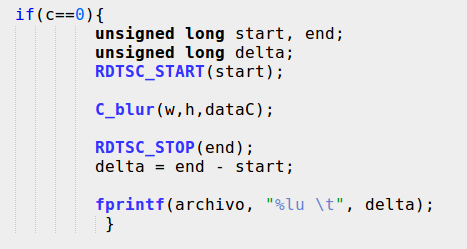
\includegraphics[width=90mm]{imagenes/resultados/codigoblur2.png}
\caption{Extracto de código modificado de run_blur en run.c.}
\end{figure}

\item {Como primera observación, el código no arrojaba los mismos resultados si realizamos 1000 iteraciones seguidas de la misma implementación en lugar de ir alternandolas. Es decir, si hacíamos 1000 ejecuciones de C, luego las 1000 de ASM1, y finalmente las 1000 de ASM2, las últimas ejecuciones del código, principalmente las de C, observamos que el tiempo que tarda en ejecutar cada iteración se vuelve menor, en parte probablemente al aprovechamiento de la cache. Para solucionar ésto, decidimos alternar la ejecución de las implementaciones, de manera que nuestro código ejecute 1 de C, 1 de ASM2, 1 de ASM2, y luego comenzar de nuevo hasta completar las 1000 iteraciones.}

\item {Una vez obtenidos los tiempos de cada iteración, usando las funciones que provee LibreCalc (Excel), calculamos la media de la muestra para cada implementación y su desvío estandar.}

\item {Para filtrar los outliers, decidimos calcular el rango determinado por la fórmula a continuación, de manera que aquellas mediciones fuera de rango, sean sacadas de la muestra. De esa manera calculamos un nuevo promedio con la "podada" de la muestra, y su nuevo desvío estandar.}

Rango aceptable para las mediciones: 
\[
(q_{1} - 3*IQR ;\ q_{3} + 3*IQR) ,\ con\ IQR = q_{3} - q_{2}
\]

\item {Para realizar las mediciones utilizamos una notebook sony VAIO con procesador Intel Core i5, 5.7gb de memoria RAM y s.o. Ubuntu 14.04 de 64bits.}

\end{itemize}


\subsection{Experimento 1}

Este primer experimento busca relacionar el rendimiento de las implementaciones de C, ASM1 y ASM2 de cada filtro, de manera general. Para ello, mostraremos en profundidad los resultados obtenidos por cada implementación para una imagen determinada, comparando con la versión no optimizada del compilador de C. (En este caso, lena.512x512.bmp, con value=0.5 en los casos del merge y hh=360, ss=0.2 y ll=0.1 en los casos del hsl.)

\begin{figure}[ht!]
\centering
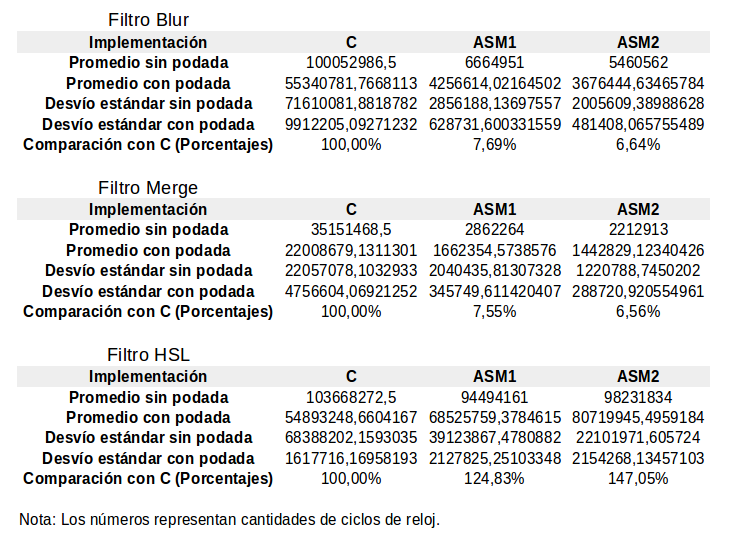
\includegraphics[width=150mm]{imagenes/resultados/tablacomparacion.png}
\caption{Tablas de Resultados para cada Implementación, 1000 iteraciones.}
\end{figure}

Como se puede notar en la tabla, para este caso, obtenemos los siguientes resultados con respecto al rendimiento de las implementaciones:

\begin{itemize}

\item { En el caso de Blur, la implementación ASM1 corre aproximadamente 13 veces más rápido que la de C, mientras que la de ASM2 corre 15 veces más rápido. Ésto es lógico pues en la segunda implementación se procesa de a 4 píxeles a la vez, mientras que en la primera se procesa de a 1 por vez, sin embargo, no es una diferencia demasiado notable, teniendo en cuenta el desvío estandar de la muestra podada. }
\item { En el caso de Merge, obtenemos aproximadamente las mismas relaciones con respecto a C. ASM1 funciona 13 veces más rápido que C, mientras que ASM2 15 veces más rápido. Ésto se debe a que al trabajar con enteros, en ASM2, nos ahorramos las conversiones a floats de los componentes, además de un paso de desempaquetado extra que no es necesario ya que podemos trabajar directamente con los words enteros. Sin embargo, al observar las imágenes resultantes, aparece una pequeña, y a nuestro criterio, aceptable pérdida de precisión. Como mucho, los componentes de la implementación en enteros varían en 1 con respecto a las otras.}
\item { Por último, en el caso de HSL, a diferencia de las anteriores, C le saca ventaja a las dos implementaciones de assembler. La de C tarda aproximadamente el 80\% de lo que tarda la de ASM1, y un 70\% de lo que tarda la de ASM2. Es decir, ASM2 es la de menor rendimiento. Existen diversos motivos que posibilitaron este resultado:
	\begin{itemize}
	\item {En principio, para las llamadas a rgbTOhsl y viceversa, fue necesario tener un vector auxiliar donde guardar los resultados de dichas funciones, haciendo que se necesite un nivel alto de accesos a memoria.}
	\item {Además, la complejidad de las conversiones, en caso de ASM2, complejizaron el algoritmo, pues en C la secuencia de ifs se resuelve de manera más rápida que de la forma en que esta implementada usando instrucciones de SIMD. En assembler, y con esta implementación, es necesario corroborar todas las condiciones de los ifs anidados, y actualizar los valores en caso de que se cumplan, a diferencia de C, en donde una vez que se cumpla una de ellas no es necesario revisar las demás. Además, para complejizar aún más, se utilizan en varias ocasiones máscaras, que se traducen en más accesos a memoria, e instrucciones de SHUFFLE para facilitar la manipulacion del orden de los componentes durante la conversión. }
	\item {Otro punto a tener en cuenta, es por ejemplo, la manera en que están implementadas las funciones fabs y fmod en C, pues en nuestra implementación fabs corresponde a un acceso a memoria y la aplicación de una máscara que modifica el bit de signo, mientras que para calcular fmod es necesario una serie de operaciones, incluida una conversión de float a entero. Ésto hace probable que éstas, y algunas otras funciones en C puedan estar implementadas más eficientemente.}
	\item {Por último, y no menos importante, las llamadas reiterativas a C en ASM1 producen overhead.}
	\end{itemize}
	}
\end{itemize}	

El siguiente gráfico muestra de manera más clara las relaciones comentadas anteriormente entre las distintas implementaciones:

\begin{figure}[ht!]
\centering
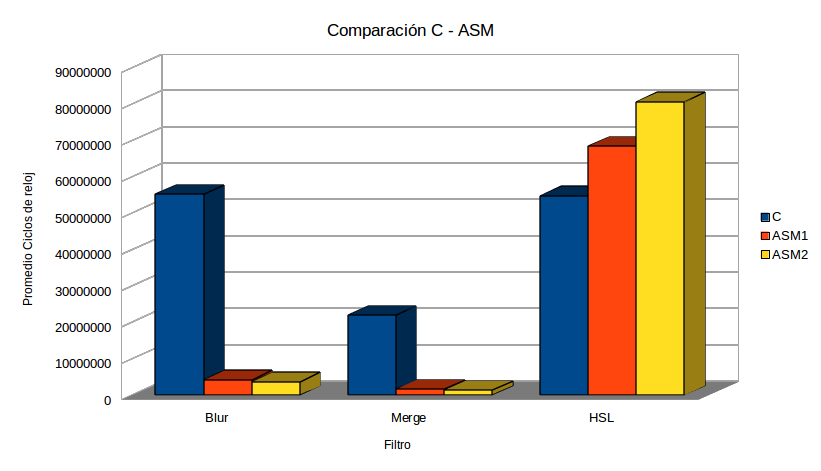
\includegraphics[width=120mm]{imagenes/resultados/graficocomparacion.png}
\caption{Gráfico de Barras, Comparación C-ASM, Experimento 1.}
\end{figure}

\newpage


\subsection{Experimento 2}

En este experimento comparamos el rendimiento de las implementaciones con respecto a los diferentes tamaños de entrada. Para ello, modificamos la imagen lena.bmp y medimos los tiempos de ejecución para cada tamaño. Decidimos hacerlo solo para Blur y Merge para ganar claridad en el gráfico, ya que los valores de los tiempos promedio de HSL difieren bastante con los de Blur y Merge.

\begin{figure}[ht!]
\centering
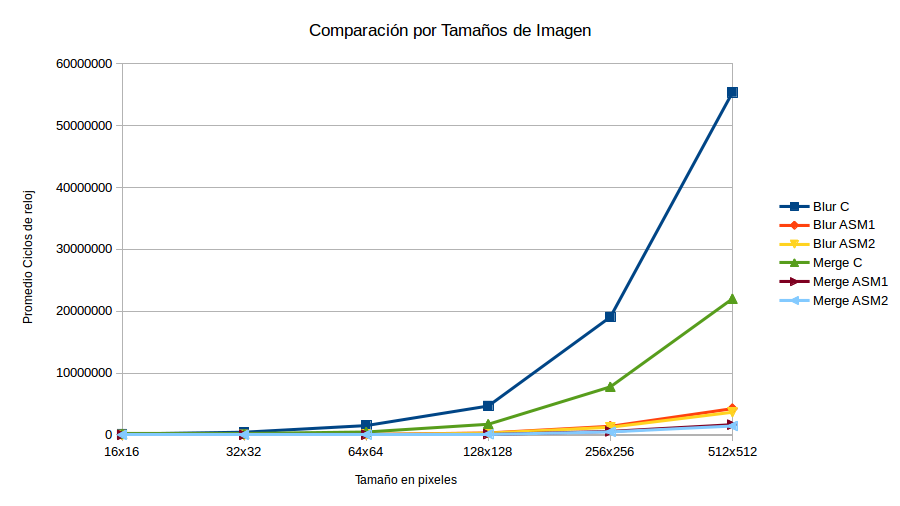
\includegraphics[width=150mm]{imagenes/resultados/graficotamanio.png}
\caption{Gráfico de Líneas, Experimento 2.}
\end{figure}

Como resultado importante, vemos que al aumentar el tamaño de la entrada (en cada punto se cuadriplica el tamaño de la imagen), la version de C crece mucho más rápido que la de ASM, es decir, la cantidad de ciclos que le toma a C procesar imágenes cada vez más grandes aumenta más velozmente que lo que le lleva a las funciones en asm. De manera que cuanto mayor es el tamaño de la imagen, más notoria es la ventaja de los programas realizados en asm. 


\subsection{Experimento 3}

En este experimento, comparamos cada implementación de los filtros contra las distintas optimizaciones posibles del compilador gcc para la version implementada en C.

\begin{figure}[ht!]
\centering
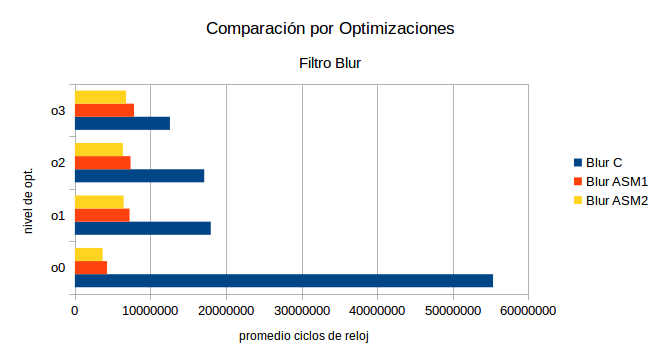
\includegraphics[width=125mm]{imagenes/resultados/grafico-opt-blur.png}
\caption{Filtro Blur, Experimento 3.}
\end{figure}

Observamos que la eficacia de los programas implementados en C depende directamente del grado de optimización con el que lo compilamos. En los casos de Blur y Merge, aún comparando con la optimizacion 3, las versiones en assembler andan más rápido que las de C, mientras que HSL de C supera  a las de ASM con más amplia claridad a medida que aumentamos el nivel de optimizacion.

\begin{figure}[ht!]
\centering
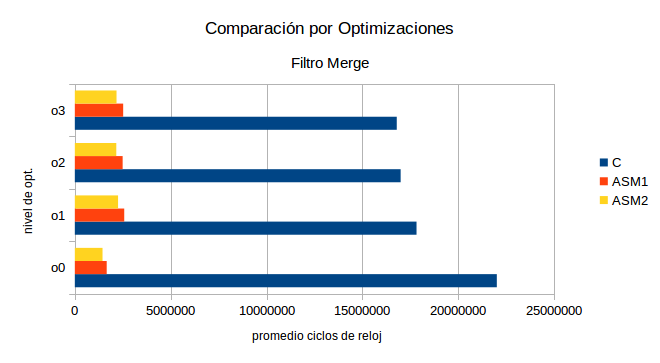
\includegraphics[width=125mm]{imagenes/resultados/grafico-opt-merge.png}
\caption{Filtro Merge, Experimento 3.}
\end{figure}

\begin{figure}[ht!]
\centering
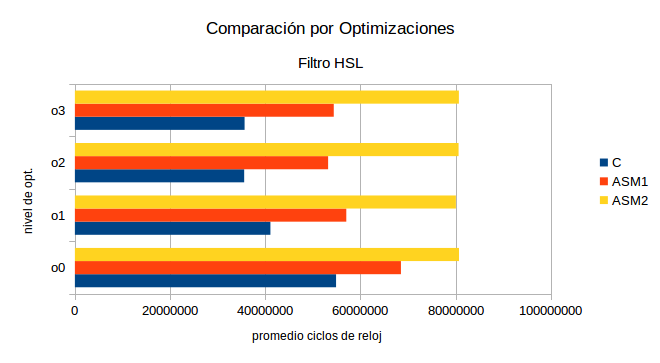
\includegraphics[width=125mm]{imagenes/resultados/grafico-opt-hsl.png}
\caption{Filtro HSL, Experimento 3.}
\end{figure}

\pagebreak
\pagebreak
\newpage

\subsection{Experimento 4}

En este experimento ejecutamos y comparamos las implementaciones con imágenes de distintos colores de fondo, siendo estos Rojo, Verde, Azul, Blanco y Negro.

\begin{figure}[ht!]
\centering
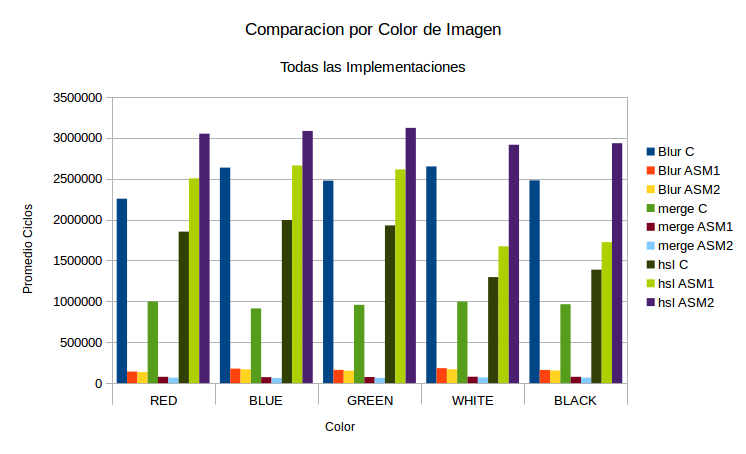
\includegraphics[width=120mm]{imagenes/resultados/grafico-colores1.png}
\caption{Comparación Filtros, Experimento 4.}
\end{figure}

Como se ve en la figura, en la mayoría de las implementaciones no se nota una diferencia importante, todas se comportan de manera similar, excepto HSL, que como se ve en detalle en la próxima figura, sus implementaciones de C y de ASM1 tardan menos con imágenes blancas o negras.

\begin{figure}[ht!]
\centering
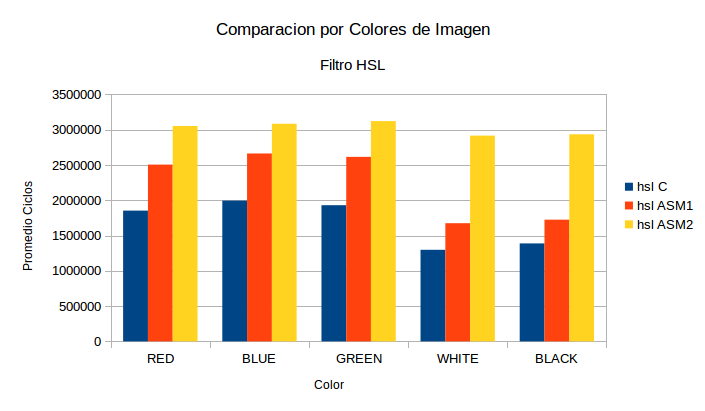
\includegraphics[width=110mm]{imagenes/resultados/grafico-colores2.png}
\caption{Comparación Filtros HSL, Experimento 4.}
\end{figure}

Ésto se debe a que para realizar las conversiones de rgb a hsl y viceversa, la complejidad del algoritmo para píxeles en blanco o negro se simplifica, ya que en ambos casos entrara en el primero de los ifs de las conversiones, sin necesidad de entrar a los else, mientras que en el ASM2 si debera ejecutar todas las ramas, reemplazando en caso de que sea necesario por el nuevo valor.
Como conclusión podemos sacar, que ASM2 corre con desventaja con respecto a ASM1 y C para todos los píxeles cuyas componentes coincidan en su valor, ya que en esos casos también se simplifica el cálculo para la conversión de un modelo a otro en la funcion de C. (Si los componentes son iguales, cmax==cmin , haciendo que el valor de h sea 0, y si al sumar queda menor de 60, cuando se convierta a RGB tambien alcanzara con el primer if, sin necesidad de ejecutar los otros).
Hay que tener en cuenta que por cada if, nuestra implementacion utiliza instrucciones de SHUFFLE, cuyos costos ifluyen directamente en el rendimiento de ASM2.

\newpage

\subsection{Experimento 5}


Como último experimento, decidimos analizar si podríamos optimizar los algoritmos reduciendo la cantidad de saltos condicionales. Para ello propusimos dos maneras de comprobar si esto valdría la pena. 
Las mediciones de este experimento se realizaron, por comodidad, sobre las implementaciones del filtro Merge.
Por un lado, medimos el promedio de 1000 iteraciones aplicando la función a dos imágenes de 32x32 y 1024x1 pixel respectivamente, de manera que ambas tienen la misma cantidad de píxeles, pero la segunda sólo entrará una vez al ciclo de filas.
Por otro lado, modificamos el algoritmo de manera que se recorra la imagen tan sólo en un ciclo, calculando la cantidad de iteraciones como el alto en píxeles de la imagen por el ancho de la imagen multiplicado por 4 (es decir, por el ancho en bytes de una fila de la imagen).

\begin{figure}[ht!]
\centering
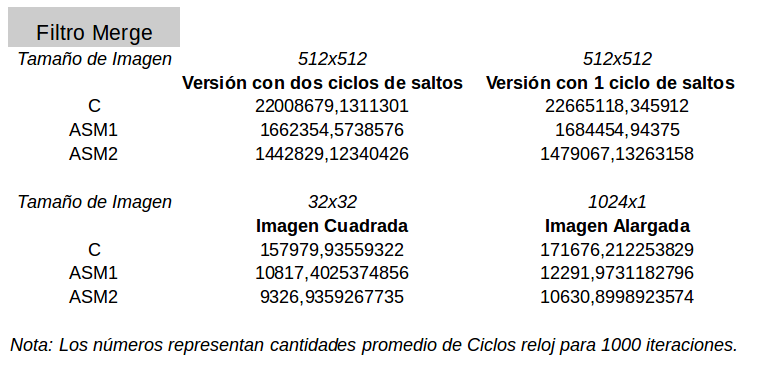
\includegraphics[width=130mm]{imagenes/resultados/tabla-saltos.png}
\caption{Resultados para Filtros Merge con menos saltos, Experimento 5.}
\end{figure}

Como se muestra en la tabla, en ambos casos no obtuvimos mejoras significativas, sino que se comportaban muy similar entre las dos. Con esto llegamos a la conclusión de que en imágenes relativamente pequeñas, utilizar 1 o 2 ciclos para recorrer la matriz no modifica la performance del algoritmo. Queda pendiente probar que sucede en mapas de bits realmente grandes, pero consideramos que estos filtros no trabajan sobre imagenes de tal tamaño.



\newpage

\section{Conclusiones}

\paragraph{} Vimos que el conjunto de instrucciones de SSE puede utilizarse para sacar provecho de la paralelización de cómputos y el acceso a memoria de a bloques de datos contiguos. Observamos que en los casos que se logró procesar más de un dato a la vez el rendimiento del algoritmo fue mayor.

\paragraph{} Además, observamos que el código de assembler generado por el compilador GCC, sin optimización, produce una gran cantidad de accesos a memoria al utilizar variables locales en la pila lo cual produce una penalización en el rendimiento del proceso. 

\paragraph{} Las circunstancias por las cuales una medición de rendimiento puede diferir de otra pueden ser muy variadas. Es importante tener en cuenta una serie de medidas para reducir al mínimo posible el error cometido, algunas de ellas utilizadas y explicadas en la sección de experimentos. Probar por nuestra cuenta y ver resultados concisos nos hizo entender mejor como maneja el procesador este tipo de operaciones, y qué tener en cuenta al momento de diseñar un algoritmo, en este caso para resolver funciones que involucran datos multimedia.


\end{document}

